
	
	


Another way to evaluate the different agents is to play against them.
To do this, we wrote a script called \texttt{human\_v\_model.py} which lets a human agent choose which model agent to play against.
Below we show what each agent's game against a human agent looked like.
For all of the images below, we tried to follow roughly the same move set so that we could see how the bots reacted differently.
The human player went first each time (X) and the agent went second (O:

First up, we will play the random agent, Charmander.
This agent will pick one of the available spaces to play using a random integer generator.
\begin{figure}[H]
	\centering
	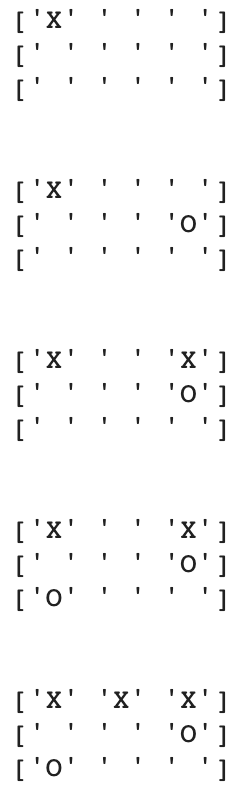
\includegraphics[scale=.5]{h_v_random}
\end{figure}
As you can see, this does not perform well.
Because it's random, it doesn't identify any potential defensive moves or offensive moves.

Next up, we will play our Dense Neural Network agent, Charmeleon.
We expect that this agent will be a stark improvement to the random agent.

\begin{figure}[H]
	\centering
	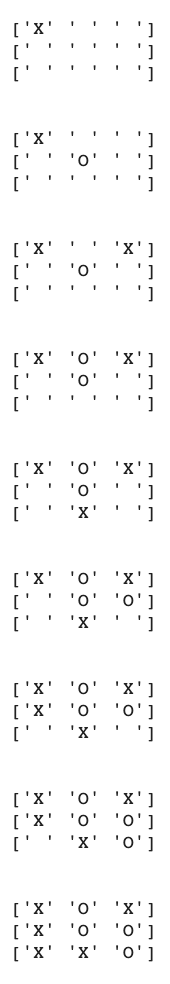
\includegraphics[scale=.5]{h_v_dense}
\end{figure}

First of all, we can see that the dense agent recognizes that it needs to play at row 1, column 2 to block the first attempt for X to win.
It then recognizes that it should play somewhere in row 2 on its next move so that it has a chance to win if X fails to block it.
If it were to play somewhere in row 3 here, it would have no chance to win.
After this move was blocked, though, is where the agent seemed to falter.
For some reason it doesn't identify that X can win in column 1 and fails to block it, resulting in the human agent winning.

Now we will play our Convolutional Neural Network agent, Charizard.
This agent performed marginally better statistically when playing the two other model agents, so we will hopefully see some better performance here.

\begin{figure}[H]
	\centering
	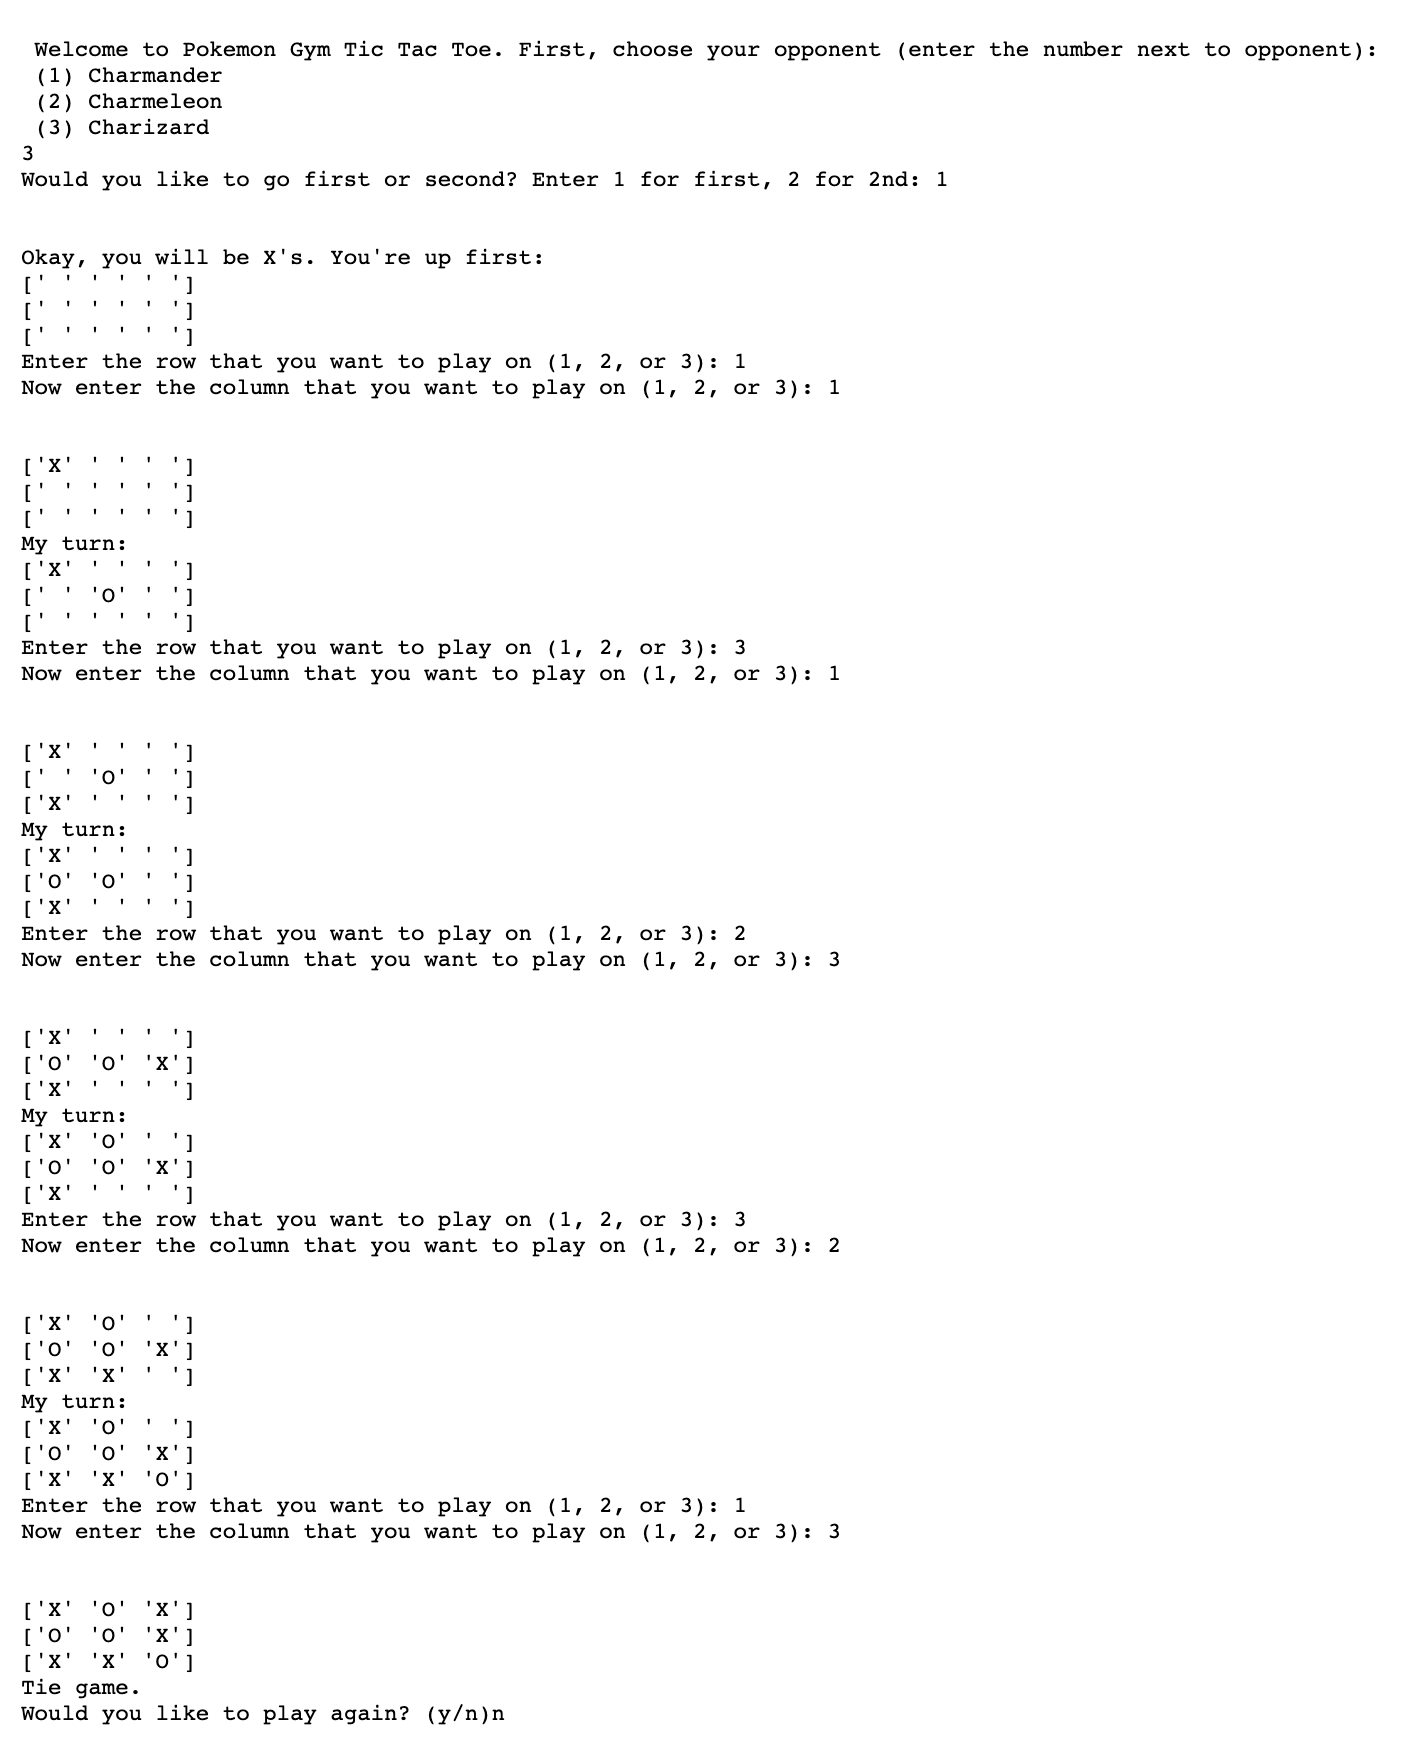
\includegraphics[scale=.5]{h_v_conv}
\end{figure}

Like the dense agent, this convolutional agent identifies and follows its best strategy early in the game.
We can see, however, that this agent correctly identifies the final chance for X to win and blocks it, resulting in a tie game.

